\clearpage
\VerdierPhysicalPageAnchor{0055}%
\VerdierSemanticAnchor{ch1-1-5-4-eq4}
由前述结果，性质 $P(\lambda,\mu)$ 在下列情形成立：

\begin{equation}
  \begin{gathered}
    \lambda\ \text{与}\ \mu\in\mathbb Z^{n-1},\\
    \lambda\ \text{与}\ \mu\in\mathbb Z e_n,\\
    \lambda\in\mathbb Z^{n-1}\ \text{且}\ \mu\in\mathbb Z e_n,\\
    \lambda\in\mathbb Z e_n\ \text{且}\ \mu\in\mathbb Z^{n-1}.
  \end{gathered}
  \tag{1.5.4.4}
\end{equation}

此外，由 (1.5.5) 得：

\VerdierSemanticAnchor{ch1-1-5-4-eq5}
\begin{quote}
  \noindent\textup{(1.5.4.5)}\quad
  \emph{若性质 $P(\mu,\nu)$、$P(\lambda+\mu,\nu)$、
  $P(\lambda,\mu+\nu)$、$P(\lambda,\mu)$ 中有三个成立，
  则第四个也成立。}
\end{quote}

\VerdierSemanticAnchor{ch1-1-5-4-conclusion}
由此可知，性质 $P(\lambda,\mu)$ 对每一对
$\lambda,\mu\in\mathbb Z^n$ 都成立，从而完成命题 (1.5.2) 的证明。

\VerdierSemanticAnchor{ch1-1-5-5}
\noindent\textbf{图 1.5.5.}\quad
我们来证明断言 (1.5.4.5)。以 $D(\lambda,\mu)$ 表示图
$\textup{(1.5.4.1)}_{\lambda,\mu}$。断言 (1.5.4.5) 的证明基于下图；
为简便起见，我们把它写在过渡同构 $c,c'$ 都是恒等态射的情形，
即群 $\mathbb Z^n$ 严格作用于范畴 $\mathcal C$ 与 $\mathcal C'$ 的情形：

\VerdierSemanticAnchor{ch1-1-5-5-tetrahedron}
\begin{center}
  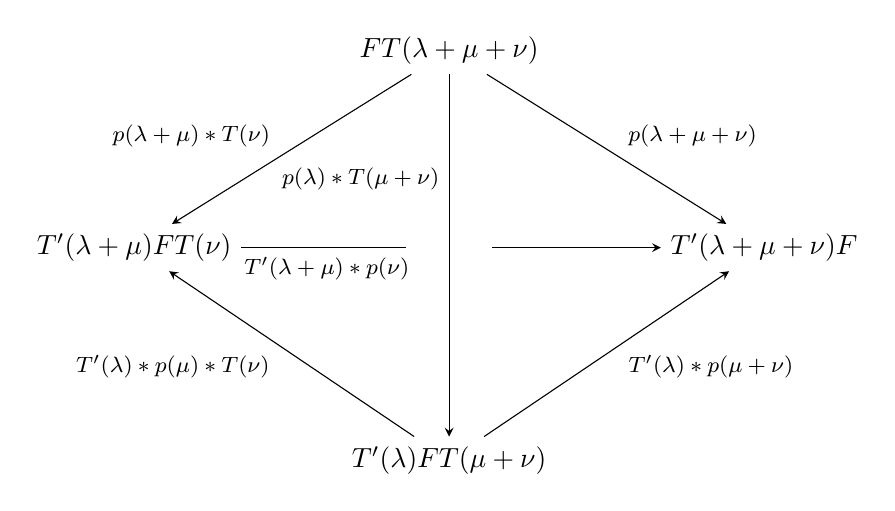
\begin{tikzpicture}[x=1cm,y=1cm,>=stealth]
    \node (a) at (0,3.2) {$FT(\lambda+\mu+\nu)$};
    \node (b) at (-4,0.7) {$T'(\lambda+\mu)FT(\nu)$};
    \node (c) at (4,0.7) {$T'(\lambda+\mu+\nu)F$};
    \node (d) at (0,-2.0) {$T'(\lambda)FT(\mu+\nu)$};
    \draw[->] (a) -- node[above left,pos=.55,font=\footnotesize]
      {$p(\lambda+\mu)*T(\nu)$} (b);
    \draw[->] (a) -- node[above right,pos=.55,font=\footnotesize]
      {$p(\lambda+\mu+\nu)$} (c);
    \draw[->] (a) -- node[left,pos=.29,font=\footnotesize]
      {$p(\lambda)*T(\mu+\nu)$} (d);
    \coordinate (bc-left) at (-0.55,0.7);
    \coordinate (bc-right) at (0.55,0.7);
    \draw (b) -- node[below,pos=.52,font=\footnotesize]
      {$T'(\lambda+\mu)*p(\nu)$} (bc-left);
    \draw[->] (bc-right) -- (c);
    \draw[->] (d) -- node[below left,pos=.55,font=\footnotesize]
      {$T'(\lambda)*p(\mu)*T(\nu)$} (b);
    \draw[->] (d) -- node[below right,pos=.55,font=\footnotesize]
      {$T'(\lambda)*p(\mu+\nu)$} (c);
  \end{tikzpicture}
\end{center}

\VerdierSemanticAnchor{ch1-1-5-5-faces}
此图呈四面体形，其四个面分别为图
$D(\lambda,\mu+\nu)$、$D(\lambda+\mu,\nu)$、
$D(\lambda,\mu)T(\nu)$ 与 $T'(\lambda)D(\mu,\nu)$。
于是考察四种可能情形并使用余循环关系，即可证明 (1.5.4.5)。

\VerdierSemanticAnchor{ch1-1-5-5-reduction}
在一般情形中，需要引入的图稍复杂一些；但利用恒等式 (1.2.1.3)，
论证可归结为上面所概述的论证。要得到 (1.5.3.5) 的证明，只需在同一图中置
\[
  \lambda=qe_1,\qquad \mu=q'e_1,\qquad \nu=q''e_1.
\]
